%%This is a standard LaTeX2e article document template. personal version 12/5/200%%
\documentclass[11pt,twoside]{article}
%%%%%%%%%%%%%%%%%%%%%%%%%%%%%%%packages%%%%%%%%%%%%%%%%%%%%%%%%%%%%%%%%%%%%%%%%%%%%%%%%%%%%%%%%%%
\pagestyle{empty}

\usepackage{latexsym}
\usepackage{amssymb}
\usepackage{amsfonts}
\usepackage{amstext}
\usepackage{amsthm}
\usepackage{amsmath}
\usepackage{multicol}
\usepackage{hyperref}
\usepackage{graphicx}
\usepackage{tikz}
\usepackage{wrapfig}
\usepackage{enumitem}

%%%%%%%%%%%%%%%%%%%%%%%%%%%%%%%formatting%%%%%%%%%%%%%%%%%%%%%%%%%%%%%%%%%%%%%%%%%%%%%%%%%%%%%%%
\setlength{\topmargin}{-.1in}        %%%  This sets all the spacing stuff to use the page more
\setlength{\oddsidemargin}{0in}    %%%  efficiently than the normal "article" setup would.
\setlength{\evensidemargin}{0in}   %%%  It's OK to play with these some.
\setlength{\textheight}{9in}     %%%
\setlength{\textwidth}{6.25in}     %%%
\setlength{\headsep}{0in}          %%%
\setlength{\headheight}{0in}       %%%
%\setlength{\footskip}{0in}         %%%
\newcommand\ord{\operatorname{ord}}
%%%%%%%%%%%%%%%%%%%%%%%%%%%%%%%%%%%%%%%%%%%%%%%%%%%%%%%%%%%%%%%%%%%%%%%%%%%%%%%%%%%%%%%%%%%%%%%

\begin{document}

\begin{center}
{\bf \Large Math 335, Homework 7}\\
\vspace{0.1in}
{\Large Due Friday, April 2 (note extended deadline!)}
\vspace{0.1cm}
\end{center}

\hrule

\vspace{.2in}

\begin{enumerate}

 \item Let
 \[H = \{e, \; (1,2)(3,4), \; (1,3)(2,4), \; (1,4)(2,3)\} \subseteq S_4.\]
 List all left cosets of $H$ in $S_4$, being sure to list each one only once..
 
{\color{red}Answer:}\\
There are $\displaystyle\frac{|S_4|}{|H|} = \frac{24}{4} = 6$ unique left cosets of $H$ in $S_4$.
\begin{center}
\begin{tabular}{ | c | c | c | c | c | c | }
\hline
$eH$ 					& $(1,2)H$ 			& $(1,3)H$ 			& $(2,3)H$ 			& $(1,2,3)H$ 			& $(1,2,4)H$ \\\hline
$e$   					& $(1,2)$   			& $(1,3)$   			& $(2,3)$    			& $(1,2,3)$   				& $(1,2,4)$ \\
$(1,2)(3,4)$   	& $(3,4)$   			& $(1,2,3,4)$   		& $(1,3,4,2)$    	& $(1,3,4)$   				& $(1,4,3)$ \\
$(1,3)(2,4)$   	& $(1,3,2,4)$   		& $(2,4)$   			& $(1,2,4,3)$    	& $(2,4,3)$   				& $(1,3,2)$ \\
$(1,4)(2,3)$  		& $(1,4,2,3)$   		& $(1,4,3,2)$   		& $(1,4)$    			& $(1,4,2)$   				& $(2,3,4)$ \\\hline
\end{tabular}
\end{center}
 
 \vspace{0.5cm}
 
 \item Let $G= \langle g \rangle$ be a cyclic group with $30$ elements.  List all of the left cosets of $\langle g^4 \rangle$ in  $G$, being sure to list each one only once.  
 
 {\color{red}Answer:}\\
There are $\displaystyle\frac{|\langle g \rangle|}{|\langle g^4 \rangle|} = \frac{30}{15} = 2$ unique left cosets of $\langle g^4 \rangle$ in $G$.  The two left cosets of $\langle g^4 \rangle$ in $G$ are:
\begin{align*}
\langle g^4 \rangle &= \{ g^2, g^4, g^6, g^8, g^{10}, g^{12}, g^{14}, g^{16}, g^{18}, g^{20}, g^{22}, g^{24}, g^{26}, g^{28}, g^{30} \}\\
g\cdot\langle g^4 \rangle &= \{ g^1, g^3, g^5, g^7, g^9, g^{11}, g^{13}, g^{15}, g^{17}, g^{19}, g^{21}, g^{23}, g^{25}, g^{27}, g^{29} \}
\end{align*}

\vspace{0.5cm}
 
 \item Let $\mathbb{C}^*$ be the group of nonzero complex numbers (under multiplication).  Recall that the {\it norm} of a complex numbers is defined as its distance from the origin in the complex plane; in other words, it's
 \[|a+bi| := \sqrt{a^2 + b^2}.\]
 Two facts about the norm, which you may assume for this problem, are
 \[|z \cdot w| = |z| \cdot |w| \;\;\; \text{ and } \;\;\; \left| \frac{1}{z} \right| = \frac{1}{|z|}.\]
 Given this, let
\[H = \left\{z \in \mathbb{C}^* \; \bigg| \; |z| = 1\right\} \subseteq \mathbb{C}^*.\]
(The next page shows a picture of $H$, for your reference.)

\begin{enumerate}

\item Prove that, for $v,w \in \mathbb{C}^*$, we have $vH = wH$ if and only if $|v| = |w|$.

\begin{proof}[\color{red}Proof.] Let $v,w \in \mathbb{C}^*$.  Suppose $vH = wH$ and $x_1,x_2 \in H$ such that $vx_1 = wx_2$.  With some algebraic manipulation, we can state that $vw^{-1} = x_2 x_1^{-1}$.  Using the properties of the norm, it can be asserted that
\[ \left\lvert  x_2 x_1^{-1} \right\rvert = \left\lvert x_2 \right\rvert \cdot \left\lvert x_1^{-1} \right\rvert = \frac{|x_2|}{|x_1|} = 1. \]
Notice that this also means that
\[ \left\lvert  v w^{-1} \right\rvert = \left\lvert v \right\rvert \cdot \left\lvert w^{-1} \right\rvert = \frac{v}{w} = 1, \]
which allows us to conclude that $\left\lvert v \right\rvert = \left\lvert w \right\rvert$.

Conversely, suppose that $\left\lvert v \right\rvert = \left\lvert w \right\rvert$ for $v,w \in \mathbb{C}^*$.  Then $\frac{|v|}{|w|} = 1$ and by using the properties of the norm, we can conclude that $\left\lvert  v w^{-1} \right\rvert = 1$.  Hence, $v w^{-1} \in H$ and $vH = wH$.
\end{proof}

\vspace{0.25cm}

\item Given part (a), draw a picture of the left coset $5H$, and of the left coset $(1+i)H$.

{\color{red}Answer:}
\begin{center}
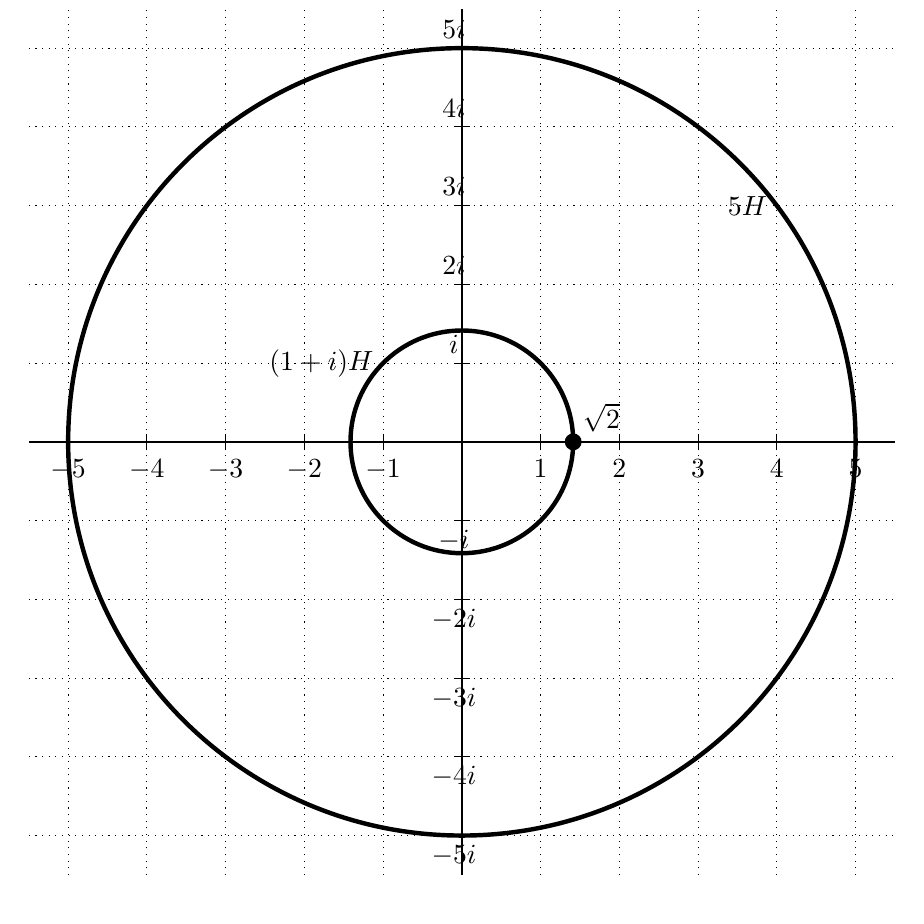
\begin{tikzpicture}[xscale=1, yscale=1]
\draw[black,thick] (-5.5, 0) -- (5.5, 0);
\draw[black,thick] (0,-5.5) -- (0, 5.5);
\draw[step=1,black,thin,dotted] (-5.5,-5.5) grid (5.5,5.5);

\draw[black, ultra thick] (0,0) circle (5);
\draw[black, ultra thick] (0,0) circle ({sqrt(2)});

\draw (5,0.1) -- (5,-0.1) node[below]{$5$};
\draw (4,0.1) -- (4,-0.1) node[below]{$4$};
\draw (3,0.1) -- (3,-0.1) node[below]{$3$};
\draw (2,0.1) -- (2,-0.1) node[below]{$2$};
\draw (1,0.1) -- (1,-0.1) node[below]{$1$};
\draw (-1,0.1) -- (-1,-0.1) node[below]{$-1$};
\draw (-2,0.1) -- (-2,-0.1) node[below]{$-2$};
\draw (-3,0.1) -- (-3,-0.1) node[below]{$-3$};
\draw (-4,0.1) -- (-4,-0.1) node[below]{$-4$};
\draw (-5,0.1) -- (-5,-0.1) node[below]{$-5$};
\draw(0.1,5) -- (-0.1,5) node[above]{$5i$};
\draw(0.1,4) -- (-0.1,4) node[above]{$4i$};
\draw(0.1,3) -- (-0.1,3) node[above]{$3i$};
\draw(0.1,2) -- (-0.1,2) node[above]{$2i$};
\draw(0.1,1) -- (-0.1,1) node[above]{$i$};
\draw(0.1,-1) -- (-0.1,-1) node[below]{$-i$};
\draw(0.1,-2) -- (-0.1,-2) node[below]{$-2i$};
\draw(0.1,-3) -- (-0.1,-3) node[below]{$-3i$};
\draw(0.1,-4) -- (-0.1,-4) node[below]{$-4i$};
\draw(0.1,-5) -- (-0.1,-5) node[below]{$-5i$};

\draw (-1,1) node[left]{$(1+i)H$};
\draw (4,3) node[left]{$5H$};
\filldraw ({sqrt(2)},0) circle (0.1cm) node[right, anchor=south west]{$\sqrt{2}$};


\end{tikzpicture}
\end{center}

\vspace{0.25cm}

\end{enumerate}

\item Let $G$ be a group with $8$ elements.

\begin{enumerate}

\item What are the possible orders of elements of $G$?

{\color{red}Answer:}\\
By corollary, the possible orders of elements of $G$ are divisors of $|G|$, which are 1, 2, 4, and 8.

\vspace{0.25cm}

\item Prove that $G$ must have an element of order $2$.

\vspace{0.1cm}

\noindent ({\bf Hint}: Start by choosing a non-identity element of $G$ at random.  If it doesn't have order $2$, try to cook up an element of order $2$ out of it.)

\begin{proof}[\color{red}Proof.]Suppose $g \in G$ and $g \neq e$.  If $\ord(g) = 8$, then $\ord(g^4) = 2$.  Similarly, if $\ord(g) = 4$, then $\ord(g^2) = 2$.  Hence, $G$ must have an element of order $2$.
\end{proof}

\vspace{0.25cm}

\end{enumerate}

\item Prove that a group with a prime number of elements must be cyclic.

\begin{proof}[\color{red}Proof.]Suppose that $\ord(G)$ is prime. Let $g \in G$ and $g \neq e$.  Since $G$ is a finite group, by corollary, $\ord(\langle g \rangle)$ divides $|G|$.  Additionally, since $g \neq e$, $\ord(\langle g \rangle) \neq 1$.  Since the only two divisors of a prime number are $1$ and itself, $\ord(\langle g \rangle) = |G|$, and it follows that $\langle g \rangle = G$.
\end{proof}

\end{enumerate}

\end{document}
